\documentclass[12pt,halfline,a4paper]{ouparticle}

\usepackage{graphicx}
\usepackage{libertine}
\usepackage[english]{babel}
\usepackage[utf8]{inputenc}
\usepackage{breakcites}
\usepackage{microtype}
\usepackage{rotating}

\usepackage[round]{natbib}

\usepackage{adjustbox}
\usepackage{booktabs,multirow,array}
\usepackage{amssymb, amsmath}
\usepackage{xfrac}
\usepackage{longtable}
\usepackage[toc,page]{appendix}

\usepackage{xcolor}
\usepackage{hyperref}
\hypersetup{
    colorlinks,
    linkcolor={red!50!black},
    citecolor={blue!30!black},
    urlcolor={blue!30!black}
}
\usepackage{lineno}
\linenumbers

\begin{document}

\title{YAMDA: A maximum likelihood hierarchical modularity detection algorithm}

\author{%
\name{Diogo Melo \thanks{Corresponding authors.}}
\address{Lewis-Sigler Institute for Integrative Genomics - Princeton University}
\email{diogro@gmail.com}
\and
\name{Fabio Machado \textup{*}}
\address{Virginia Polytechnic Institute and State University, VT - Department of Biological Sciences}
\email{macfabio@gmail.com}
%\and
%\name{Gabriel Marroig}
%\address{Departamento de genética e biologia evolutiva, Instituto de Biociências, Universidade de São Paulo, São Paulo, SP, Brasil}
%\email{gmarroig@usp.br}
}

\abstract{\textbf{
Multivariate quantitative
genetics provides a powerful framework for understanding patterns and
processes of phenotypic evolution. Quantitative genetics parameters,
like trait heritability or the G-matrix for sets of traits, can be used
to predict evolutionary response or to understand the evolutionary
history of a population.}}

\date{\today}

\keywords{G-matrix; modularity; phenotypic correlation; factor analysis}

\maketitle

\section*{Introduction}

Phenotypes are the result of many overlaping genetic effects and developmental
processes \citep{Lande1983-ez,Klingenberg2008-ll,Melo2016-yw}. These different
factors create a structured pattern of phenotypic correlations, which we can
measure and use to infer something about the underlying processes. Identifing
modules, groups of traits that are more related among themselves than with other
traits, is a powerful way to describe and interpret the patterns of pheotypic
covariation.

Discussion on overlapping factors contributing to covariation (Mitteroecker2007,
Hallgrimsson2012)

Several methods for assessing the apropriatness of putative modularity
hypothesis exist in the literature. These methods use variations on some comon
themes, like hypothesis testing and model comparison.

Brief review of existing methods:

\begin{itemize}
    \item CR    
    \item EMMLi
    \item Mint
    \item Mantel
\end{itemize}

Most methods of comparing different modularity hypothesis don't allow for the
comparison of nested hypothesis. 

Most are ad-hock measures similarity, and do
not allow for the use of proper statistical methods. 

The likelihood in EMMLi is
extrapolated from the expectation on measuring the correlation between two
traits, and does not acctually use the data in the likelihood computation, only
the correlations. 

Yamda sets it self appart by using the likelihood of the data to compare the
different modularity hypothesis, allowing for overlaping modules, allowing
different methods for the construction of the putative covariance matrix, and
having 


\begin{figure}[h]
    \center
    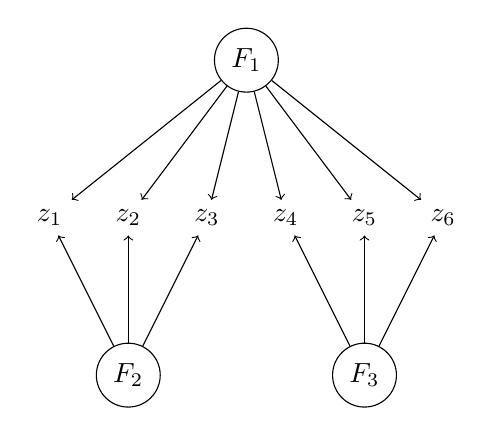
\begin{tikzpicture}
    \node[draw, circle] (F1) at (2.5,2) {$F_1$};
    \node[draw, circle] (F2) at (1,-2) {$F_2$};
    \node[draw, circle] (F3) at (4,-2) {$F_3$};

    \node (z1) at (0,0) {$z_1$};
    \node (z2) at (1,0) {$z_2$};
    \node (z3) at (2,0) {$z_3$};
    \node (z4) at (3,0) {$z_4$};
    \node (z5) at (4,0) {$z_5$};
    \node (z6) at (5,0) {$z_6$};

    \draw [->] (F1) edge (z1) (F1) edge (z2) (F1) edge (z3) 
               (F1) edge (z4) (F1) edge (z5) (F1) edge (z6);
    \draw [->] (F2) edge (z1) (F2) edge (z2) (F2) edge (z3);
    \draw [->] (F3) edge (z4) (F3) edge (z5) (F3) edge (z6);
\end{tikzpicture}


\caption[Factors and modules]{ Factors can overlap in their effect on traits }
\label{fig:factor-diagram}
\end{figure} 

\section*{Methods}


\subsection*{A maximum likelihood for the modularity hypothesis}

\subsection*{Carnivora sample}


\section*{Results}


\begin{figure}[h]
\includegraphics[width=5cm]{example-image-golden}
\caption[Factors and modules]{ Modulues are cool }
\label{fig:example-fig}
\end{figure}



\section*{Discussion}

The interaction between selection and multivariate covariation is a
central part of our understanding of evolution. Even simple selection
regimes can produce complex multivariate responses due to cascading
developmental effects and genetic constraints. Here, ...


\begin{notes}[Acknowledgments]
We thank Tiago Zahn for insightful discussions that contributed to the
development of this work.
\end{notes}

\begin{notes}[Funding]
This work was supported by grants...
\end{notes}


\bibliography{refs}

\bibliographystyle{apalike}

\newpage

\appendix* \section*{Supporting Information}

\makeatletter
\renewcommand{\thefigure}{S\arabic{figure}}
\makeatother

\setcounter{figure}{0}

\begin{figure}
	\includegraphics[width=10cm]{example-image-b}
`	\caption[This result in necessary but not cool.]{}
\label{fig:supporting_1}
\end{figure}


\end{document}
